\subsection{Break‐Even Penetration Analysis}
\label{sec:Results_BreakEven}

The break-even study identifies the combinations of traffic volume and \ac{mpr} for which \ac{eco-glosa} yields lower mean \ac{co2} emissions than (i) the \ac{flow-glosa} baseline and (ii) the uncontrolled Standard. The numerical results are listed in Tables~\ref{tab:BreakEven_EcoVsFlow} and \ref{tab:BreakEven_EcoVsStd}, while the decision maps are grouped in Figs.~\ref{fig:BE_EcoFlow} and \ref{fig:BE_EcoStd}.

\paragraph{\ac{eco-glosa} versus \ac{flow-glosa}.}
Under HBEFA4, the advantage of \ac{eco-glosa} shrinks as either \ac{mpr} or volume increases. For example, Table~\ref{tab:BreakEven_EcoVsFlow} shows a peak benefit of $+2.30\,\mathrm{g\,km^{-1}}$ at $69\,\mathrm{veh/h}$ and $20\%$ \ac{mpr}; thereafter values oscillate and turn negative beyond $50\%$ penetration. The transition is visible in Fig.~\subref{fig:BE_EcoFlow_HBEFA4}: the green region disappears above the dashed line, indicating that \ac{flow-glosa} becomes preferable once either traffic exceeds $500\,\mathrm{veh/h}$ or penetration surpasses $60\%$. 
\mynewline
PHEMlight5 produces a cleaner separation (Fig.~\subref{fig:BE_EcoFlow_PHEM}): \ac{eco-glosa} dominates below the grey envelope and cedes the advantage above it. Positive margins reach $+8.46$ at $346\,\mathrm{veh/h}$ and $10\%$ penetration, but fall to $-44.15\,\mathrm{g\,km^{-1}}$ at $3462\,\mathrm{veh/h}$ and $20\%$. The steeper penalty for high-demand stems from PHEMlight5’s transient engine map, which amplifies the fuel cost of the sharp accelerations induced by \ac{eco-glosa} when queues build up. A secondary insight is that the break-even curve is almost vertical between $30$ and $60\%$, implying that once penetration exceeds approximately $35\%$ the volume threshold shifts abruptly from $1000$ to $1500\,\mathrm{veh/h}$ with little sensitivity to further penetration increases.

\paragraph{\ac{eco-glosa} versus Standard.}
Figures~\ref{fig:BE_EcoStd} reveal that \ac{eco-glosa} can still outperform the uncontrolled scenario even when it loses to the baseline. For HBEFA4 (Fig.~\subref{fig:BE_EcoStd_HBEFA4}) low and medium volumes show sizeable gains, peaking at $+22.11\,\mathrm{g\,km^{-1}}$ for $69\,\mathrm{veh/h}$ and $40\%$ \ac{mpr}. The green zone narrows with demand and vanishes entirely once a stable jam exists above $2300\,\mathrm{veh/h}$. Under PHEMlight5 (Fig.~\subref{fig:BE_EcoStd_PHEM}) the usable region widens: positive differences appear for almost every \ac{mpr} above $30\%$ up to $1385\,\mathrm{veh/h}$, reaching $+24.06\,\mathrm{g\,km^{-1}}$ at $69\,\mathrm{veh/h}$ and $50\%$ \ac{mpr}. Only the two highest volumes show across-the-board detriment, with a worst case of $-163.38\,\mathrm{g\,km^{-1}}$ at $2769\,\mathrm{veh/h}$ and $60\%$ penetration.

\paragraph{Supplementary Findings.}
\begin{enumerate}
  \item \textit{Optimal penetration depends on demand.}  When traffic is light (below $500\,\mathrm{veh/h}$), each additional \ac{eco-glosa} vehicle delivers its greatest marginal emission reduction in the $10$–$30\%$ penetration range, because the algorithm can smooth vehicle arrivals without creating new stop-go waves. However, once volumes exceed $1000\,\mathrm{veh/h}$, meaningful gains only appear after $50\%$–$80\%$ of vehicles are equipped, since low to moderate penetration fails to overcome the inherent congestion dynamics. In practice, this means that planners deploying \ac{eco-glosa} should prioritise corridors with light to medium load for early rollout, while high-volume arterials require near-universal adoption before benefits materialize.
  \item \textit{Demand amplifies penalties more than partial coverage.}  Negative outcomes (where \ac{eco-glosa} increases emissions) escalate much more rapidly with rising traffic than with penetration rate. For example, at fixed $30\%$ penetration the worst-case CO$_2$ penalty under HBEFA4 grows from about $-19\,\mathrm{g/km}$ at $69\,\mathrm{veh/h}$ to over $-351\,\mathrm{g/km}$ at $3462\,\mathrm{veh/h}$, a nearly $19\times$ increase. By contrast, doubling penetration from $30\%$ to $60\%$ at moderate demand only doubles the penalty magnitude. Thus, network demand is the dominant factor in whether \ac{eco-glosa} will underperform, and flow-based control (\ac{flow-glosa}) is preferable whenever traffic approaches saturation.
\end{enumerate}

\paragraph{Implications for deployment.}
\begin{itemize}
  \item For urban volumes below $700\,\mathrm{veh/h}$, \ac{eco-glosa} becomes beneficial once penetration exceeds roughly $30\%$ (HBEFA4) or $20\%$ (PHEMlight5), offering up to $22\,\mathrm{g\,km^{-1}}$ reduction over the Standard.
  \item In the transition range ($700$–$2000\,\mathrm{veh/h}$) the algorithm should only be chosen at high penetration ($\geq80\%$); otherwise \ac{flow-glosa} is preferable, saving up to $44\,\mathrm{g\,km^{-1}}$ relative to \ac{eco-glosa}.
  \item In saturated corridors ($>2300\,\mathrm{veh/h}$) \ac{flow-glosa} is consistently superior, as its throughput maximisation suppresses stop–go oscillations that dominate fuel use.
\end{itemize}

These thresholds outline the general envelope of traffic volumes and equipment rates within which \ac{eco-glosa} can deliver emission savings, and indicate that beyond this region the throughput‐focused \ac{flow-glosa} is the more reliable choice.  

\begin{figure}[htb]
  \centering
  \begin{subfigure}[b]{0.45\textwidth}
    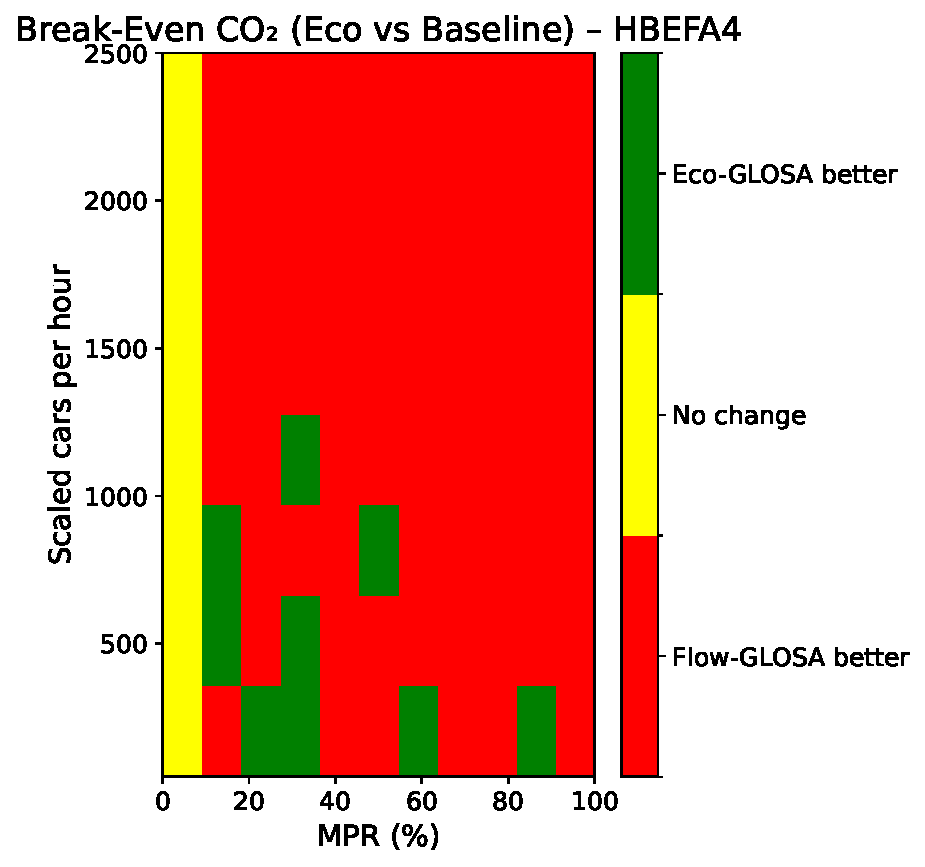
\includegraphics[width=\textwidth]{data/img/BreakEven/BreakEven_CO2_HBEFA4.pdf}
    \caption{HBEFA4 model.}
    \label{fig:BE_EcoFlow_HBEFA4}
  \end{subfigure}\hfill
  \begin{subfigure}[b]{0.45\textwidth}
    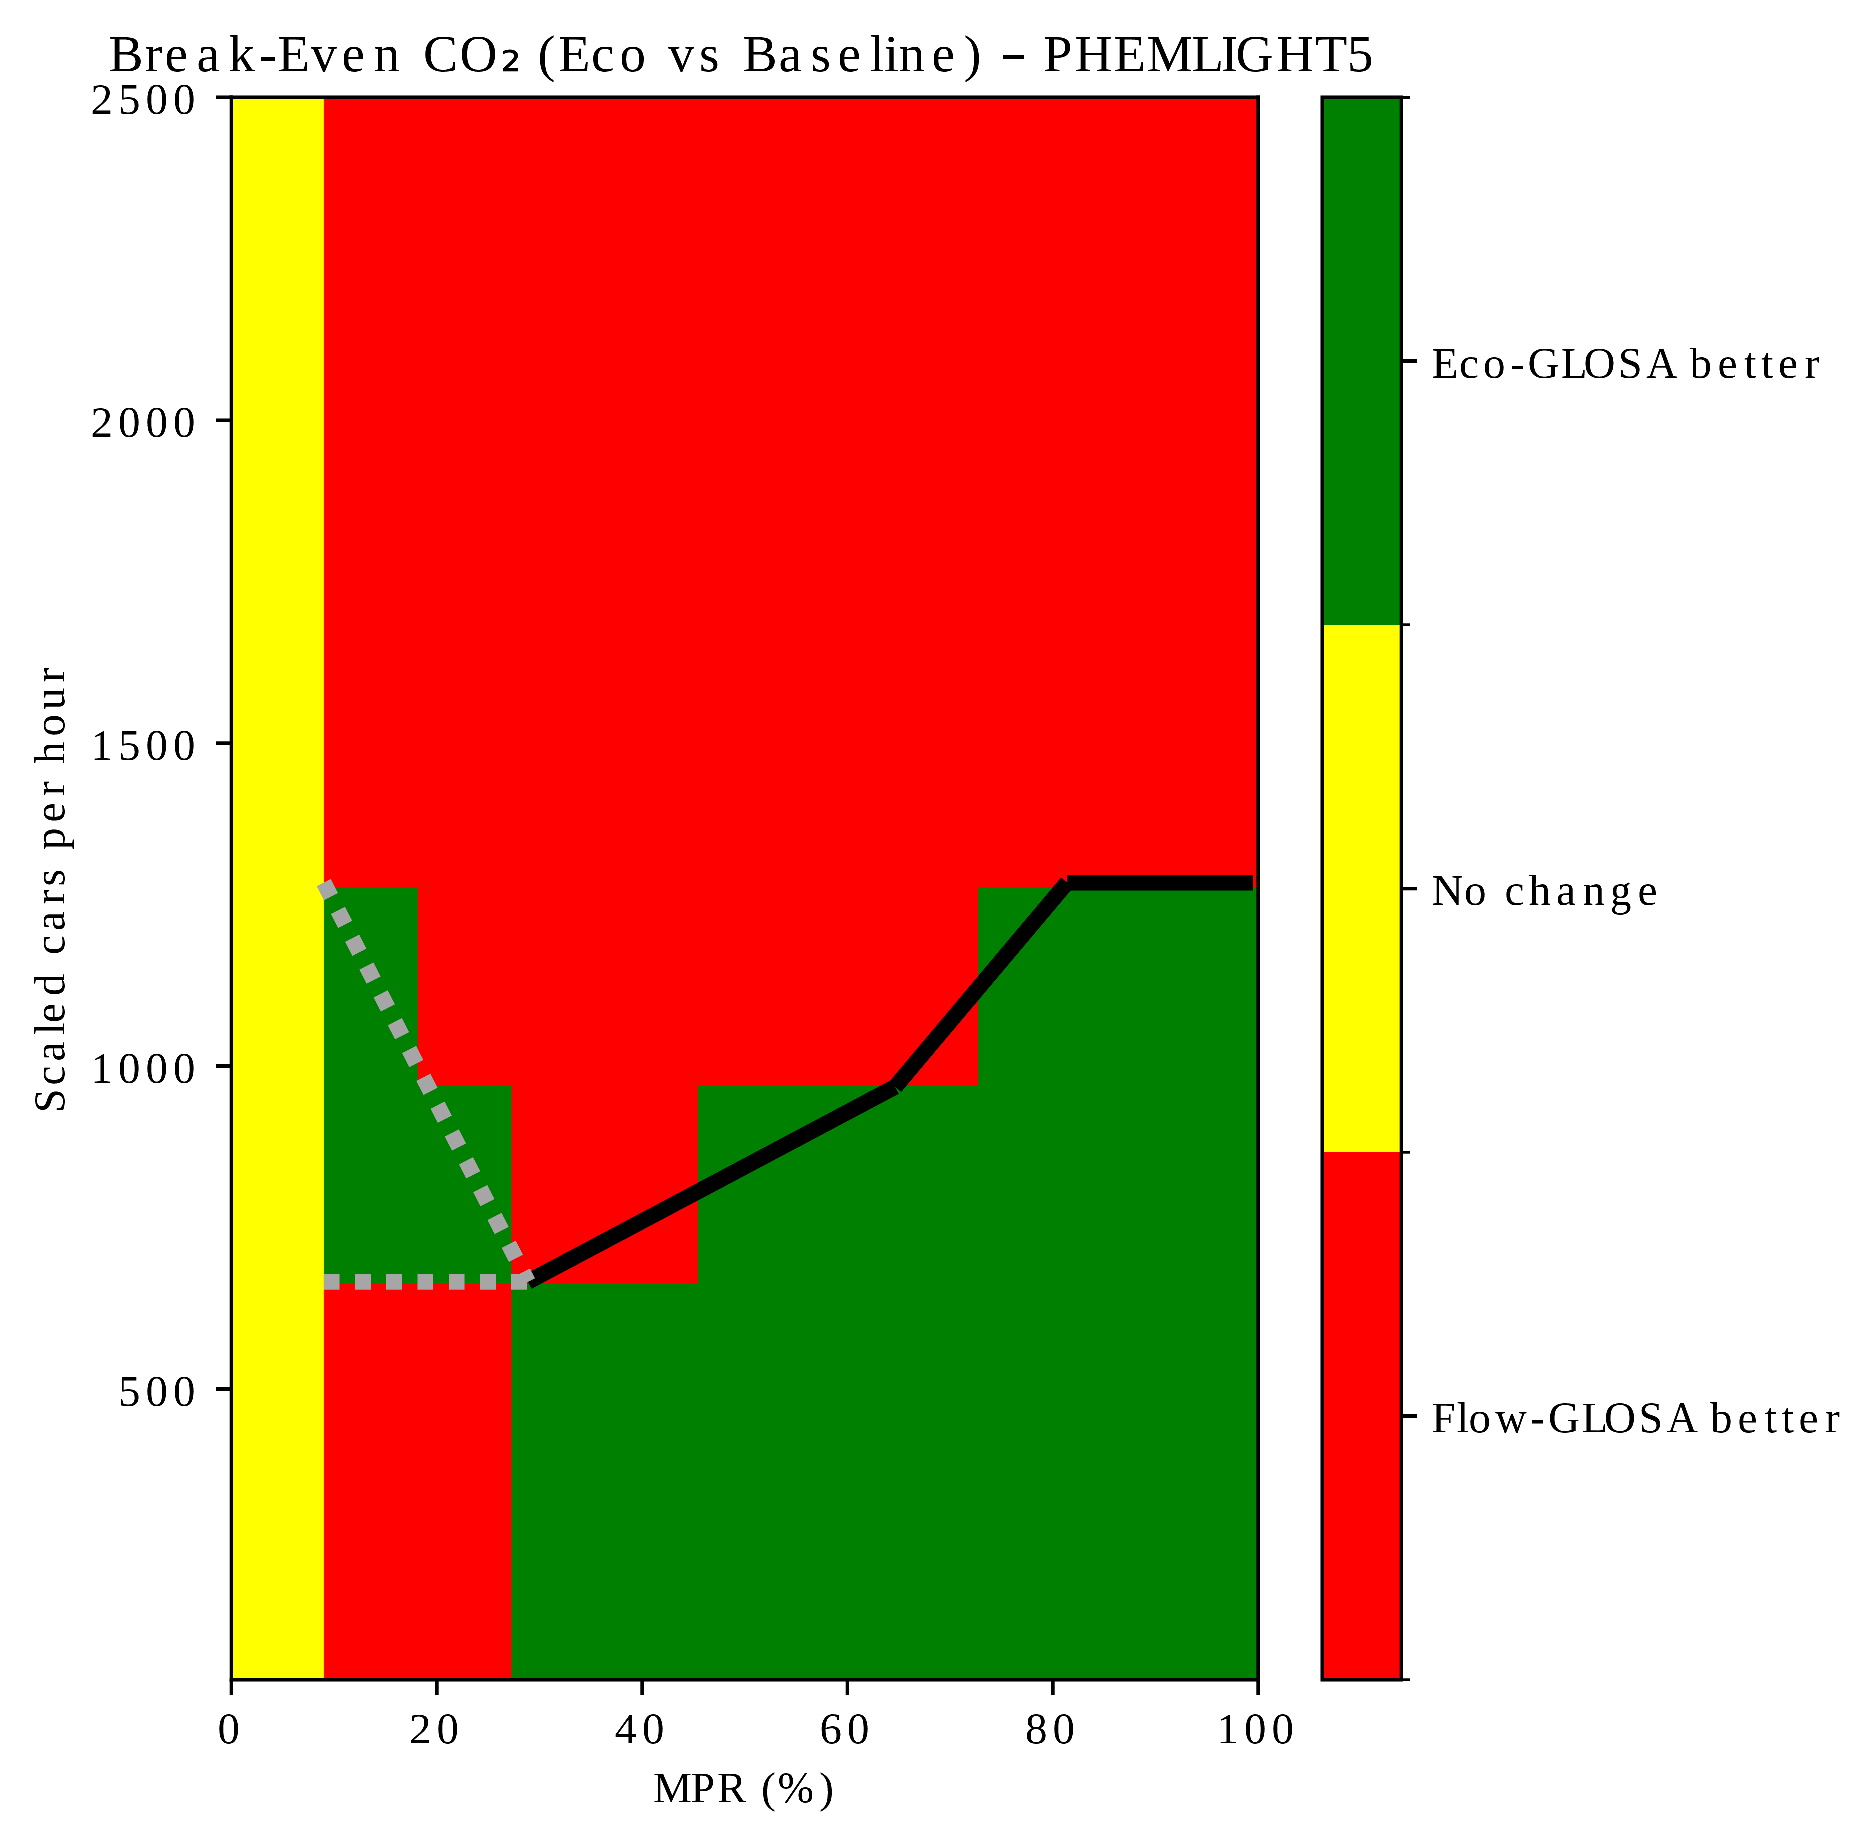
\includegraphics[width=\textwidth]{data/img/BreakEven/BreakEven_CO2_PHEMLIGHT5.pdf}
    \caption{PHEMlight5 model.}
    \label{fig:BE_EcoFlow_PHEM}
  \end{subfigure}
  \caption{Break-even CO$_2$ emission map showing the difference between \ac{eco-glosa} and \ac{flow-glosa}. Green regions indicate parameter combinations where \ac{eco-glosa} yields lower CO$_2$ emissions than \ac{flow-glosa}, while red regions denote scenarios where the baseline is more effective. Grey dashed lines represent the empirical boundary between advantageous regimes, and the solid black curve connects the points of maximum CO$_2$ benefit.}
  \label{fig:BE_EcoFlow}
\end{figure}

\begin{figure}[htb]
  \centering
  \begin{subfigure}[b]{0.45\textwidth}
    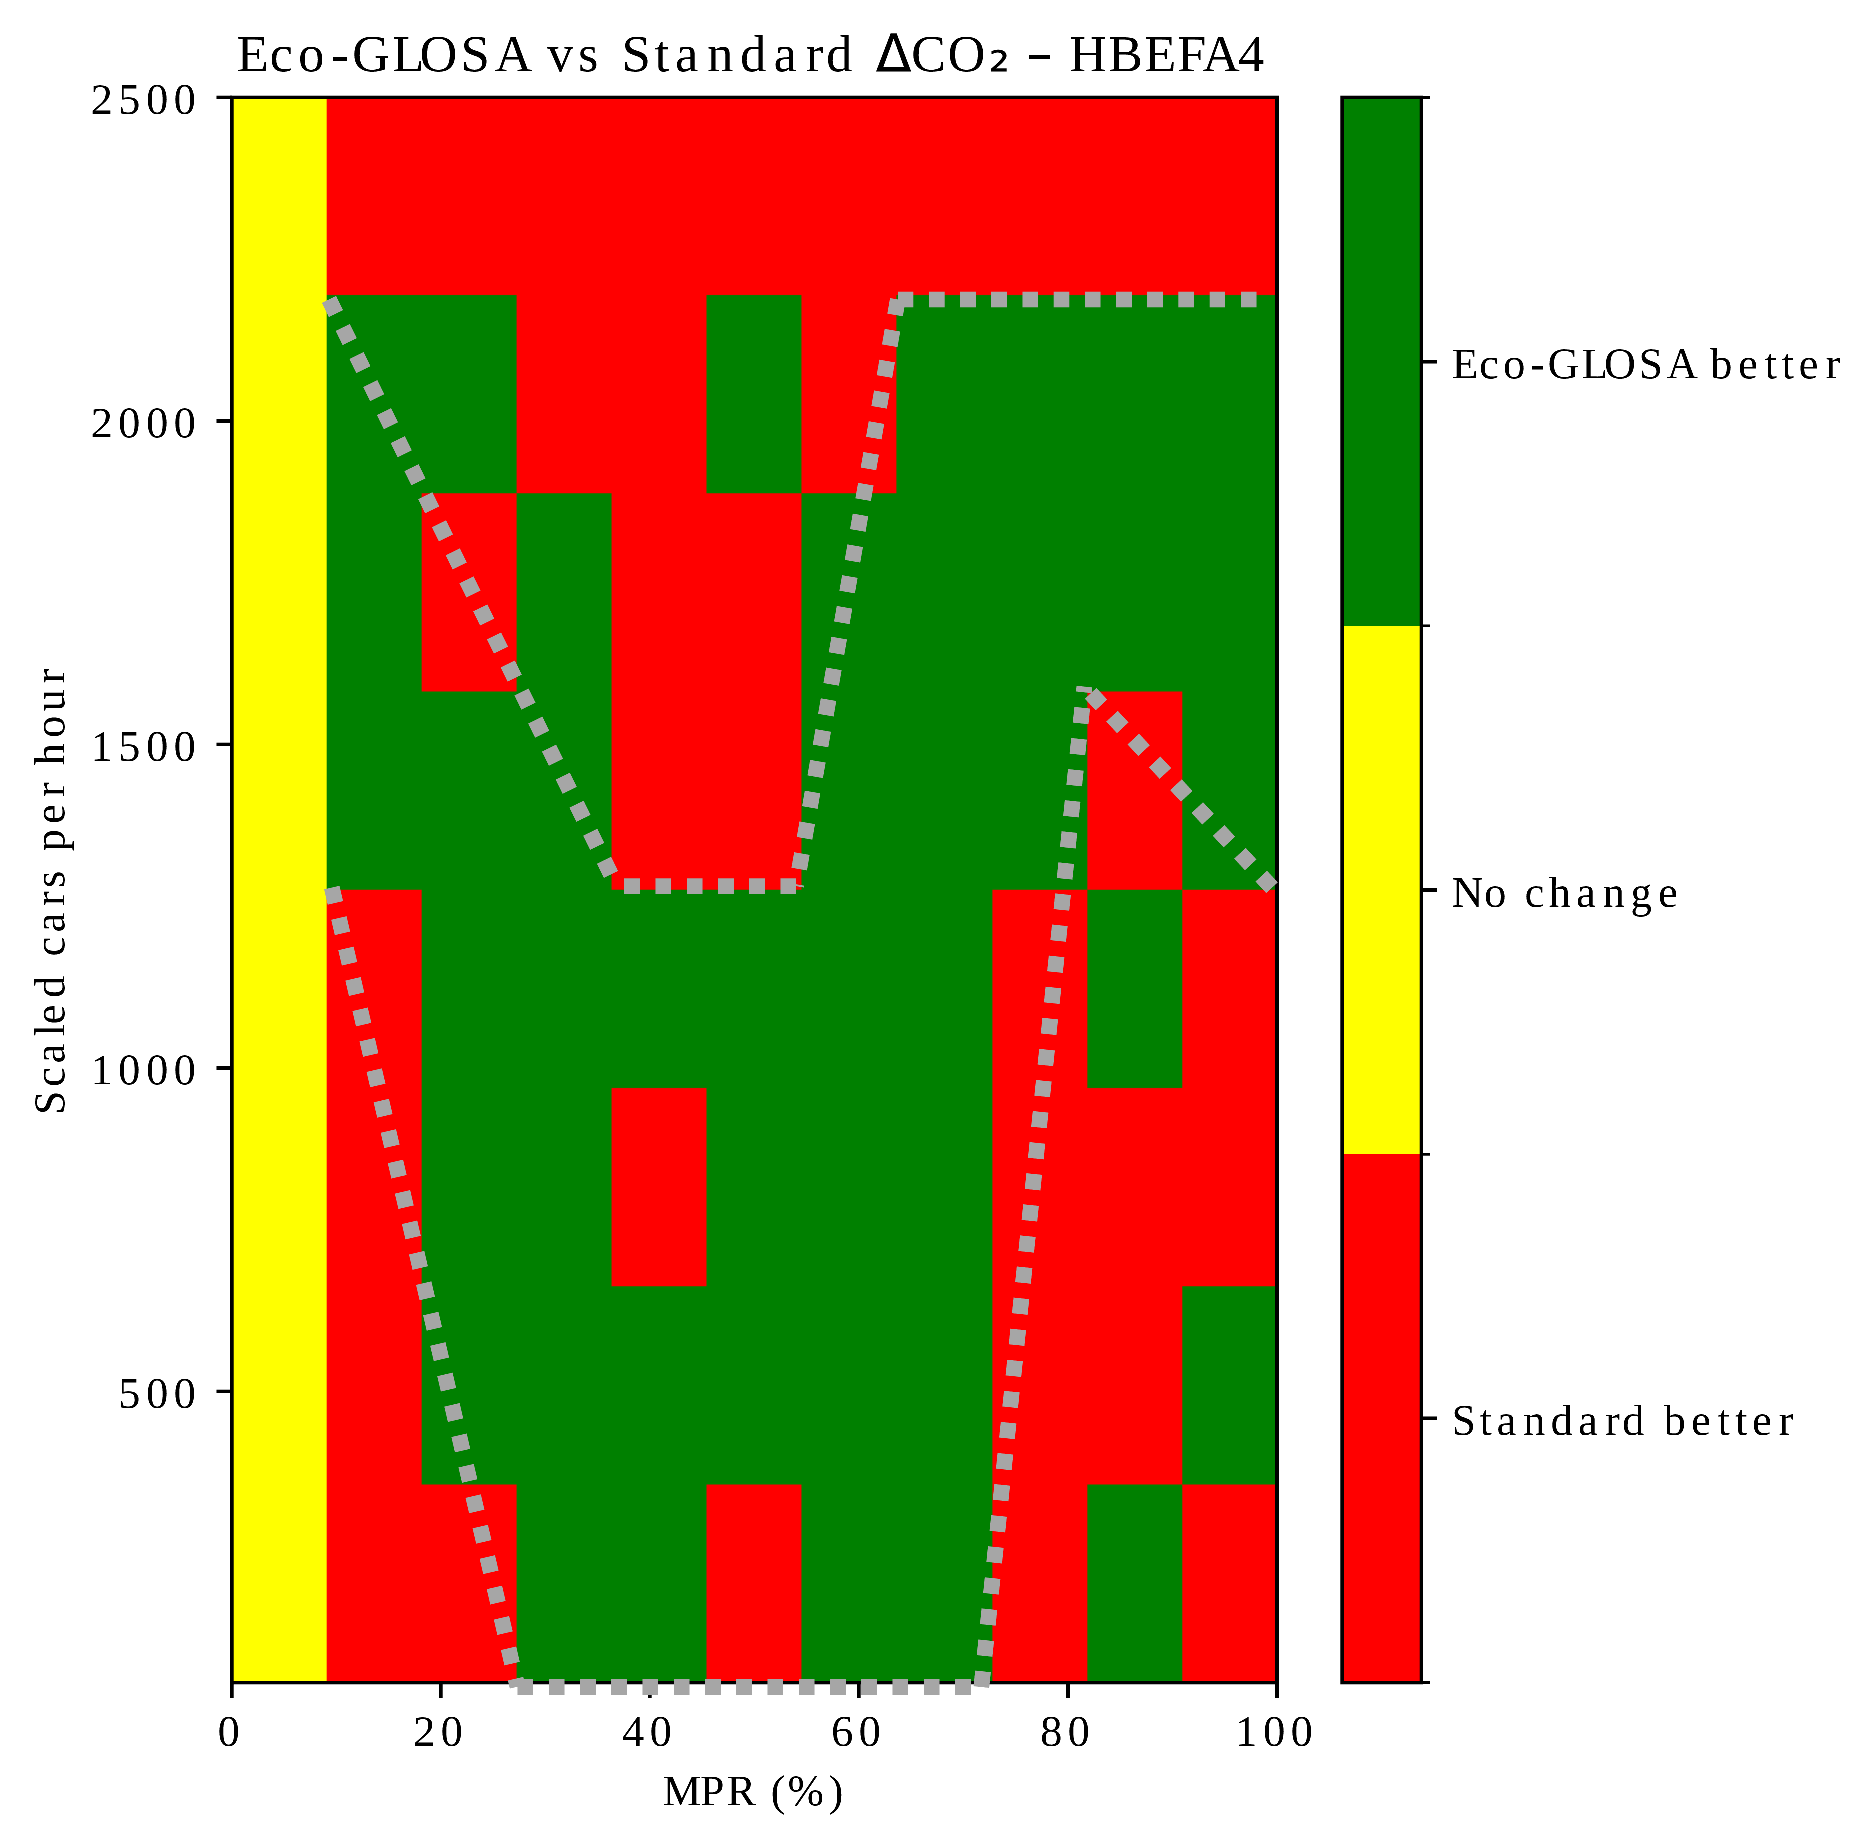
\includegraphics[width=\textwidth]{data/img/BreakEven/delta_CO2_HBEFA4.pdf}
    \caption{HBEFA4 model.}
    \label{fig:BE_EcoStd_HBEFA4}
  \end{subfigure}\hfill
  \begin{subfigure}[b]{0.45\textwidth}
    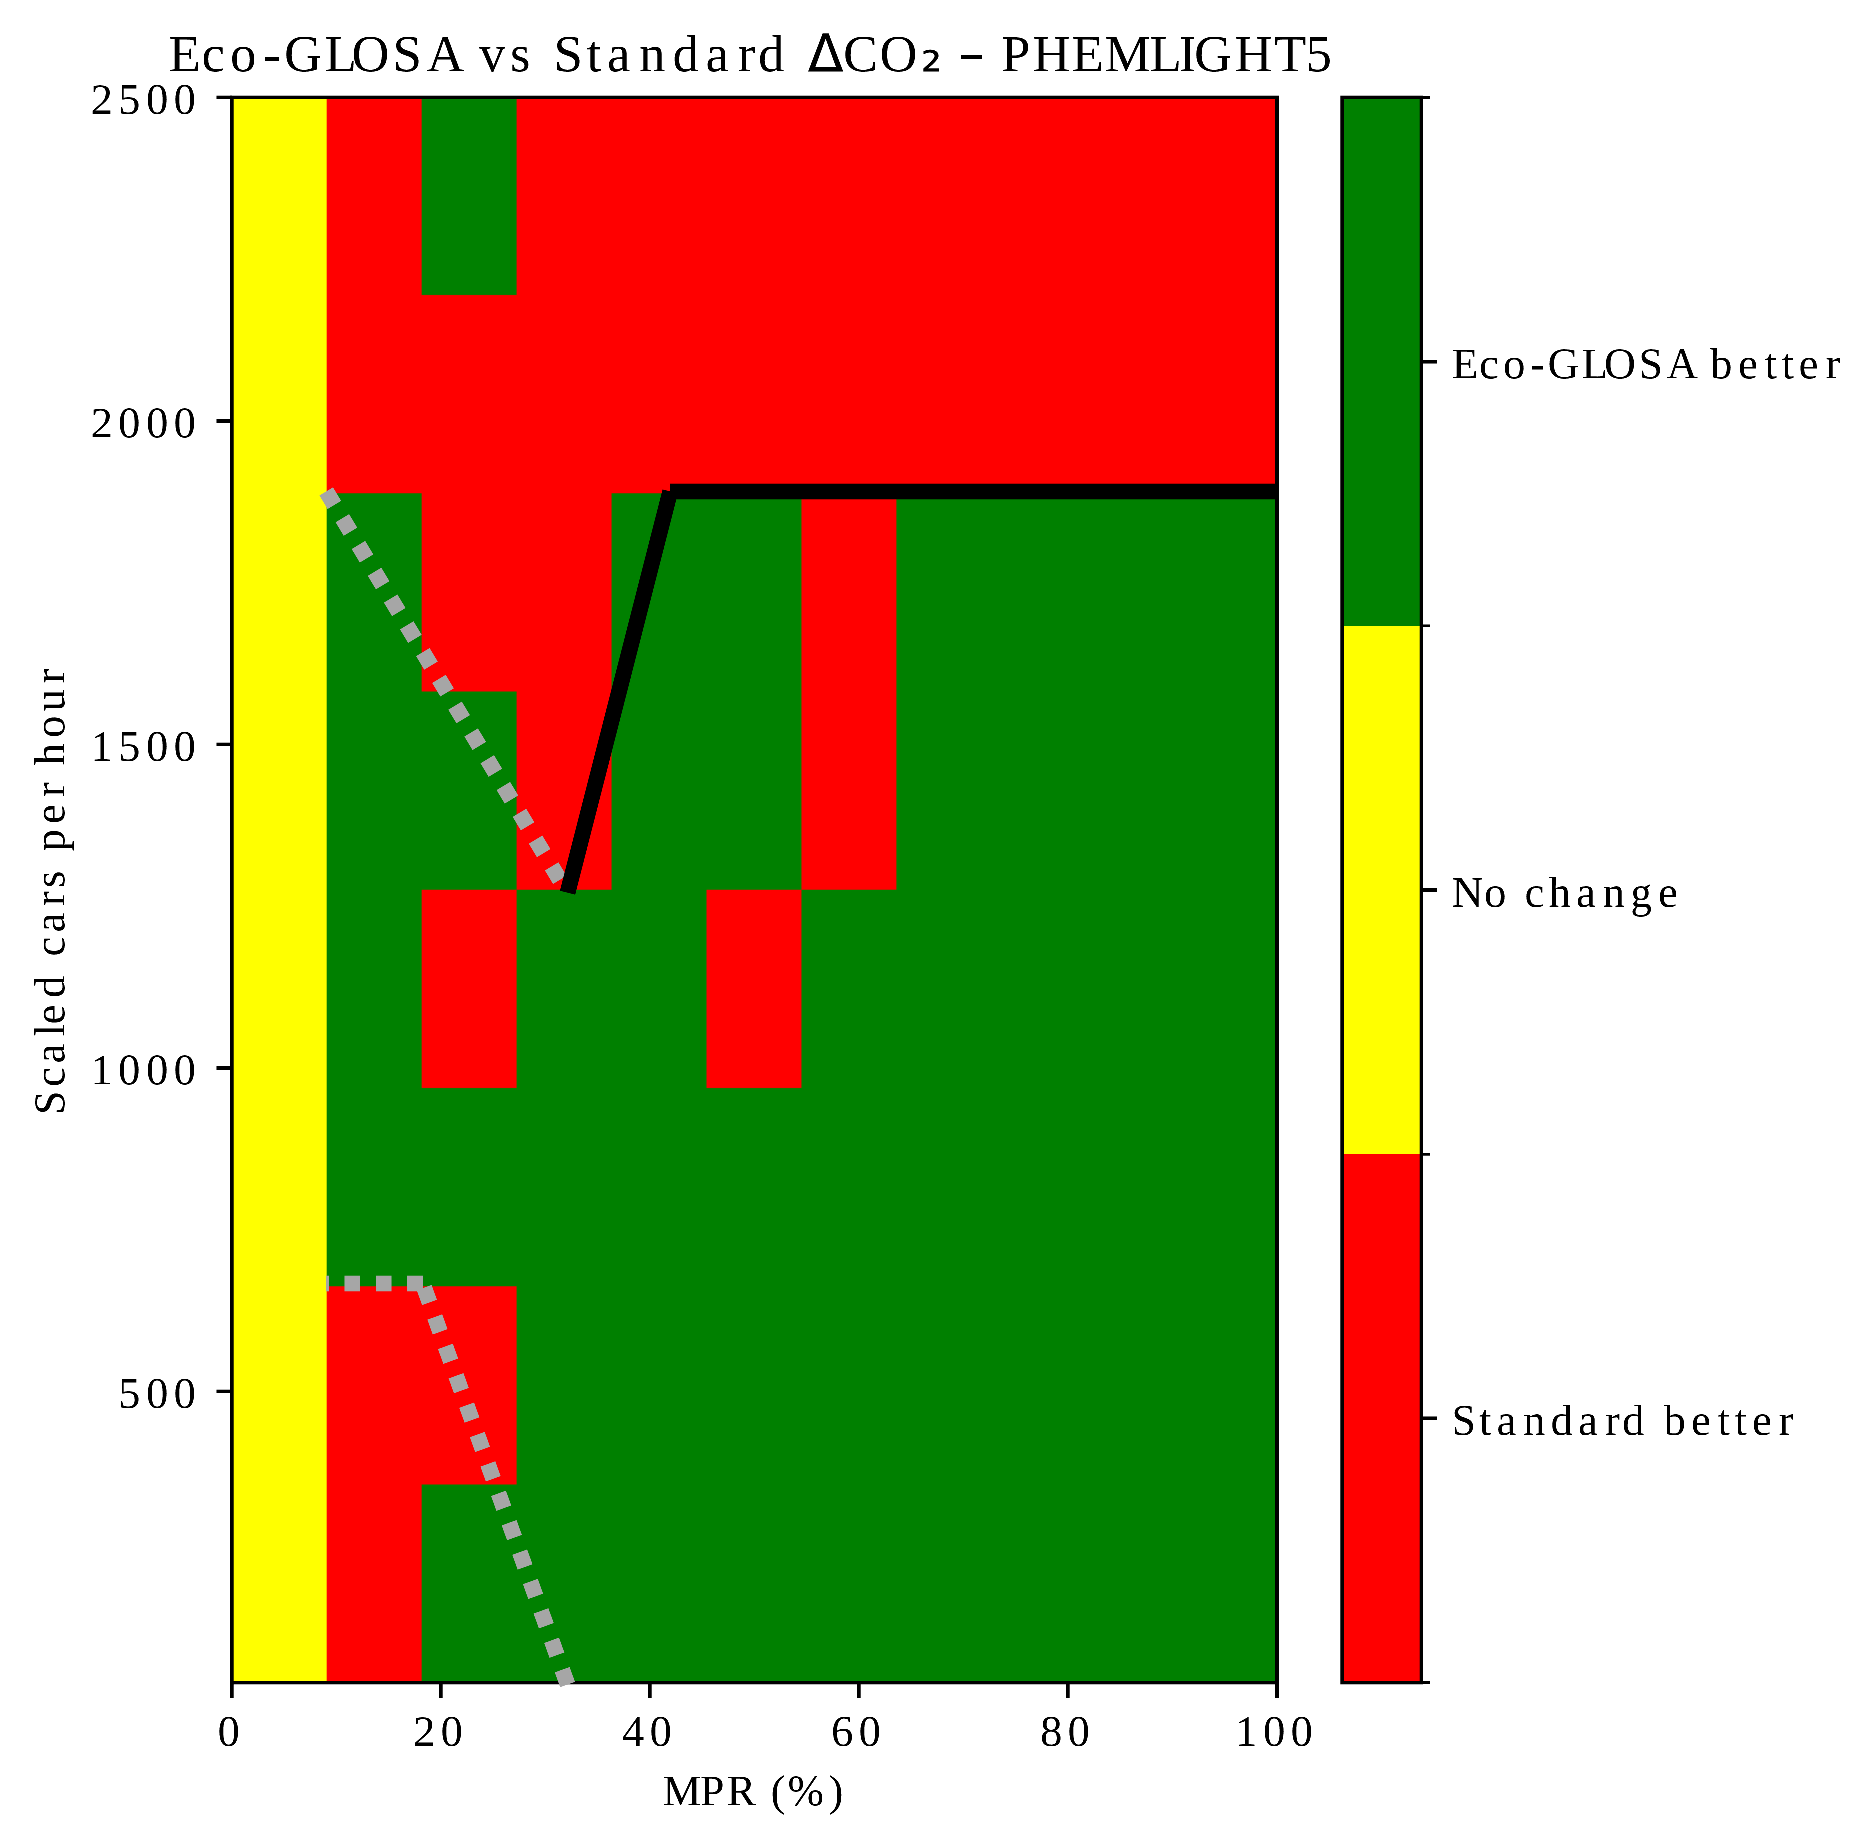
\includegraphics[width=\textwidth]{data/img/BreakEven/delta_CO2_PHEMLIGHT5.pdf}
    \caption{PHEMlight5 model.}
    \label{fig:BE_EcoStd_PHEM}
  \end{subfigure}
  \caption{Relative CO$_2$ emission reduction achieved by \ac{eco-glosa} compared to the Standard scenario (no \ac{glosa}). Green regions denote positive emission savings, while red regions indicate higher emissions relative to the Standard. Grey dashed envelopes delineate the empirically determined range in which \ac{eco-glosa} is effective; the solid black curve traces the optimal path of maximum emission reduction.}
  \label{fig:BE_EcoStd}
\end{figure}

\begin{table}[htb]
  \centering
  \caption{Break‐even analysis: CO$_2$ difference (g/km) between \ac{eco-glosa} and \ac{flow-glosa}. Positive values indicate \ac{eco-glosa} outperforms \ac{flow-glosa}.}
  \label{tab:BreakEven_EcoVsFlow}
  \resizebox{\textwidth}{!}{%
    \begin{tabular}{r l *{12}{r}}
      \toprule
      Cars & Fuel       & \textbf{0\% (Standard)} & 10\%    & 20\%    & 30\%      & 40\%      & 50\%     & 60\%       & 70\%    & 80\%    & 90\%    & 100\%   \\
      \midrule
      69   & HBEFA4     & \textbf{149.99}      & \textbf{0.53}   & \textbf{2.30}   & \textbf{0.68}   & \textbf{0.65}   & –3.55   & \textbf{1.63}    & –0.61  & –0.42  & –2.22  & –3.40  \\
      138  & HBEFA4     & \textbf{148.70}      & –6.45  & \textbf{0.26}   & \textbf{1.40}   & –4.20  & \textbf{1.84}  & –0.13   & –0.71  & –4.62  & 5.52   & 0.48   \\
      346  & HBEFA4     & \textbf{147.86}      & –1.66  & \textbf{2.19}   & –1.48  & –1.24  & \textbf{0.76}  & –0.22   & –1.16  & –2.95  & –1.48  & 0.35   \\
      692  & HBEFA4     & \textbf{148.06}      & \textbf{11.68}  & \textbf{1.07}   & \textbf{0.10}   & –0.98  & \textbf{1.02}  & –0.85   & –1.26  & –5.69  & –2.06  & –5.38  \\
      1385 & HBEFA4     & \textbf{149.86}      & \textbf{0.74}   & –0.39  & –0.71  & –1.84  & –0.37   & –2.18   & –2.01  & –0.66  & \textbf{0.97}   & –2.12  \\
      2077 & HBEFA4     & \textbf{152.91}      & \textbf{0.11}   & –2.97  & –2.38  & –0.79  & –4.25   & –3.62   & –2.82  & –1.65  & –1.73  & –4.13  \\
      2769 & HBEFA4     & \textbf{158.44}      & –5.23  & –1.99  & \textbf{–118.09} & –68.76 & –3.67   & \textbf{–272.42} & –4.30  & –3.51  & –2.69  & –3.91  \\
      3462 & HBEFA4     & \textbf{426.68}      & –54.38 & –88.56 & –102.44 & –134.41 & –157.82 & \textbf{–351.31} & –206.47 & –421.00 & –444.57 & –430.41 \\
      \midrule
      69   & PHEMlight5 & \textbf{155.51}      & –6.14  & –0.03  & \textbf{2.14}   & \textbf{2.65}   & \textbf{7.32}  & \textbf{1.26}    & \textbf{3.35}   & \textbf{1.32}   & \textbf{4.86}   & \textbf{16.51} \\
      138  & PHEMlight5 & \textbf{155.28}      & –4.94  & –2.09  & \textbf{3.63}   & \textbf{1.92}   & \textbf{4.39}  & \textbf{1.87}    & 0.51   & \textbf{6.64}   & \textbf{8.21}   & 2.86   \\
      346  & PHEMlight5 & \textbf{156.60}      & \textbf{8.46}   & \textbf{4.50}   & –0.15  & –2.59  & 0.13    & 0.39    & \textbf{1.46}   & \textbf{2.32}   & \textbf{6.19}   & 1.92   \\
      692  & PHEMlight5 & \textbf{157.36}      & 7.99   & –1.86  & –1.02  & –0.91  & –0.11   & \textbf{ –0.60} & –0.06  & \textbf{6.77}   & 1.69   & \textbf{4.51}  \\
      1385 & PHEMlight5 & \textbf{159.38}      & –1.46  & –3.82  & –4.83  & –4.89  & –4.80   & –6.19   & –3.65  & –5.33  & –0.86  & –1.36  \\
      2077 & PHEMlight5 & \textbf{162.83}      & –4.06  & –7.78  & –5.57  & –3.13  & –5.57   & –7.11   & –7.15  & –6.80  & –4.14  & –5.60  \\
      2769 & PHEMlight5 & \textbf{168.29}      & –30.19 & –69.10 & –138.25 & –125.33 & –148.94 & –172.00  & –189.98 & –142.67 & –167.68 & –104.93 \\
      3462 & PHEMlight5 & \textbf{344.88}      & –32.33 & –44.15 & –63.07  & –59.73  & –72.32  & –197.81  & –112.43 & –208.07 & –207.66 & –215.19 \\
      \bottomrule
    \end{tabular}%
  }
\end{table}

\begin{table}[htb]
  \centering
  \caption{Break‐even analysis: CO$_2$ difference (g/km) between \ac{eco-glosa} and Standard. Positive values indicate a reduction relative to the Standard.}
  \label{tab:BreakEven_EcoVsStd}
  \resizebox{\textwidth}{!}{%
    \begin{tabular}{r l *{12}{r}}
      \toprule
      Cars & Fuel       & \textbf{0\% (Standard)} & 10\%    & 20\%    & 30\%     & 40\%     & 50\%    & 60\%    & 70\%     & 80\%     & 90\%     & 100\%    \\
      \midrule
      69   & HBEFA4     & \textbf{149.99}      & –14.06 & –19.38 & \textbf{5.40}  & \textbf{22.11} & –15.56 & \textbf{6.54}  & \textbf{8.50}  & –4.29  & \textbf{2.17}  & –3.21  \\
      138  & HBEFA4     & \textbf{148.70}      & –9.72  & \textbf{5.89}  & \textbf{4.56}  & \textbf{6.55}  & \textbf{17.52} & \textbf{6.74}  & \textbf{8.11} & –13.27 & –14.47 & \textbf{2.02} \\
      346  & HBEFA4     & \textbf{147.86}      & –18.14 & \textbf{12.48} & \textbf{0.38}  & –5.30  & \textbf{16.25} & \textbf{4.94}  & \textbf{3.72} & –11.59 & –20.20 & –14.62 \\
      692  & HBEFA4     & \textbf{148.06}      & –20.25 & \textbf{1.82}  & \textbf{2.27}  & \textbf{8.91}  & \textbf{4.30}  & \textbf{5.07}  & \textbf{5.04} & –18.90 & \textbf{4.05}  & –13.03 \\
      1385 & HBEFA4     & \textbf{149.86}      & \textbf{11.98} & \textbf{8.69}  & \textbf{1.87}  & –0.86  & –3.83 & \textbf{4.40}  & \textbf{5.52} & \textbf{18.81} & –17.86 & \textbf{19.47} \\
      2077 & HBEFA4     & \textbf{152.91}      & \textbf{11.59} & –19.04 & \textbf{1.85}  & –5.16  & –4.66 & \textbf{5.54}  & \textbf{7.28} & \textbf{20.04} & \textbf{7.24}  & \textbf{19.61} \\
      2769 & HBEFA4     & \textbf{158.44}      & \textbf{8.76}  & \textbf{8.17}  & –112.49 & –65.49 & \textbf{14.37} & –260.65 & \textbf{9.24}  & \textbf{21.50} & \textbf{20.97} & \textbf{23.50} \\
      3462 & HBEFA4     & \textbf{426.68}      & –51.87 & –89.47 & –94.30  & –97.72 & –100.28 & –148.47 & –140.95 & –149.41 & –180.79 & –155.06 \\
      \midrule
      69   & PHEMlight5 & \textbf{155.51}      & –0.69  & \textbf{6.68}  & \textbf{7.14}  & \textbf{12.53} & \textbf{24.06} & \textbf{6.34}  & \textbf{10.97} & \textbf{17.26} & \textbf{19.01} & \textbf{17.94} \\
      138  & PHEMlight5 & \textbf{155.28}      & –0.40  & –7.12  & \textbf{5.37}  & \textbf{3.62}  & \textbf{11.02} & \textbf{6.47}  & \textbf{7.53}  & \textbf{5.15}  & \textbf{18.88} & \textbf{12.87} \\
      346  & PHEMlight5 & \textbf{156.60}      & \textbf{13.56} & \textbf{9.07}  & \textbf{0.79}  & \textbf{3.14}  & \textbf{8.81}  & \textbf{4.65}  & \textbf{5.37}  & \textbf{13.14} & \textbf{15.01} & \textbf{13.25} \\
      692  & PHEMlight5 & \textbf{157.36}      & \textbf{0.44}  & –9.96  & \textbf{0.16}  & \textbf{3.34}  & –5.65  & \textbf{3.85}  & \textbf{4.51}  & \textbf{13.50} & \textbf{13.52} & \textbf{18.50} \\
      1385 & PHEMlight5 & \textbf{159.38}      & \textbf{2.69}  & \textbf{0.52}  & –3.61 & \textbf{2.69}  & \textbf{1.37}  & –1.32  & \textbf{1.80}  & \textbf{5.31}  & \textbf{8.89}  & \textbf{11.17} \\
      2077 & PHEMlight5 & \textbf{162.83}      & \textbf{0.59}  & –2.37  & –3.25 & \textbf{0.84}  & \textbf{3.24}  & –0.05  & \textbf{0.80}  & \textbf{5.37}  & \textbf{10.65} & \textbf{8.52}  \\
      2769 & PHEMlight5 & \textbf{168.29}      & –23.10 & –63.72 & –135.11 & –115.95 & –137.81 & –163.38 & –179.44 & –127.66 & –153.08 & –87.61 \\
      3462 & PHEMlight5 & \textbf{344.88}      & –16.50 & \textbf{1.68}  & –54.31 & –12.24 & –24.62 & –63.75 & –65.57 & –20.02 & –14.53 & –22.90 \\
      \bottomrule
    \end{tabular}%
  }
\end{table}
